\begin{savequote}[75mm]
The imagination of nature is far, far greater than the imagination of man.
\qauthor{Richard Feynman}
\end{savequote}

\chapter{Observation of Vector Boson Fusion production of $H\rightarrow WW^{*}\rightarrow \ell\nu\ell\nu$}

\section{Introduction}

After the discovery of a particle consistent with the Higgs boson, the $\HWW$ analysis had two main goals. The first goal was to increase the sensitivity of the analysis to fully confirm that the $\HWW$ process did indeed exist. The second goal was to characterize the particle as much as possible, including searching for the lower cross-section production modes, in order to confirm that it was indeed a Higgs boson.   This chapter presents a dedicated search for Vector Boson Fusion (VBF) production of a Higgs boson decaying via the \HWWfull mode. First, basics of the topology of VBF production are presented. Then, the details of the analysis are shown, including signal region definition, background estimation techniques, and systematic uncertainties. Finally, the results of the analysis are shown. As will be shown, this analysis is the first and most sensitive observation of the VBF production mode of the Higgs on ATLAS.

\section{Topology of VBF $\HWW$ production}

As discussed in Chapter 1, the characteristic feature of VBF production of the Higgs is the presence of two additional forward jets coming from the incoming partons which radiate the vector bosons that make the Higgs. These jets are forward because the outgoing partons still carry the longitudinal momentum of the incoming partons. Figure~\ref{fig:VBF_LeadJetEta} shows the distribution of the $\eta$ for the leading jet in a VBF event compared to a background top pair production event. As can be seen, the VBF jets tend to be more forward in $\eta$, while the $\ttbar$ jets are more central. 

\begin{figure}
  \vspace{20pt}
  \centering
  \hspace*{-32pt}
  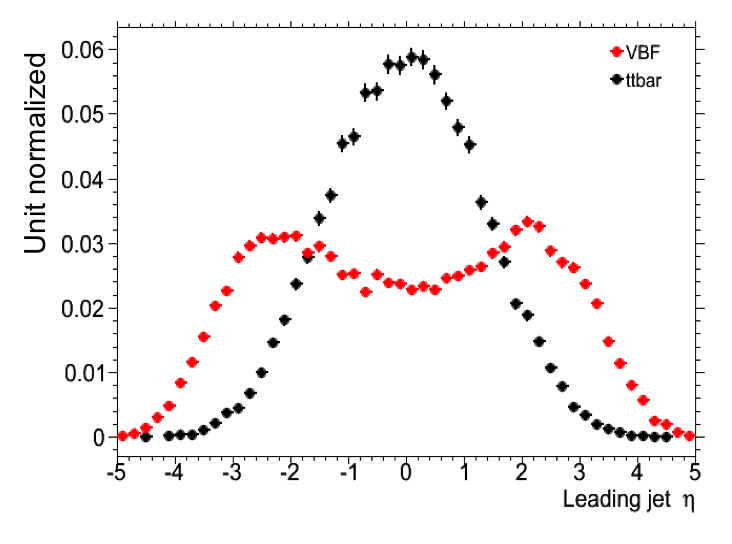
\includegraphics[width=0.6\textwidth]{figures/VBF_LeadJetEta}
  \caption{Leading jet $\eta$ in VBF $\HWW$ (red) and $\ttbar$ (black)}
  \label{fig:VBF_LeadJetEta}
\end{figure}

Because the cross section for VBF production is about an order of magnitude smaller than gluon fusion production, these forward jets must be used in order to better reduce background and achieve a good signal to background ratio. The analysis selection is constructed to maximally exploit the features of the unique VBF topology. 

\section{Data and simulation samples}

The results presented here are with 20.3 \ifb taken at $\sqrt{s} = 8 \TeV$ and 4.5 \ifb taken at $\sqrt{s} = 7 \TeV$. 

\section{Object selection}

\section{Analysis selection}

\section{Background estimation}

\section{Systematic uncertainties}

\section{Results}
